\documentclass[tikz]{standalone}
\usepackage{contour}
\usepackage[normalem]{ulem}
\usetikzlibrary{shapes,arrows.meta}
\renewcommand{\ULdepth}{1.8pt}
\contourlength{0.6pt}
\newcommand{\myuline}[1]{%
    \uline{\phantom{#1}}%
    \llap{\contour{white}{#1}}%
}
\begin{document}
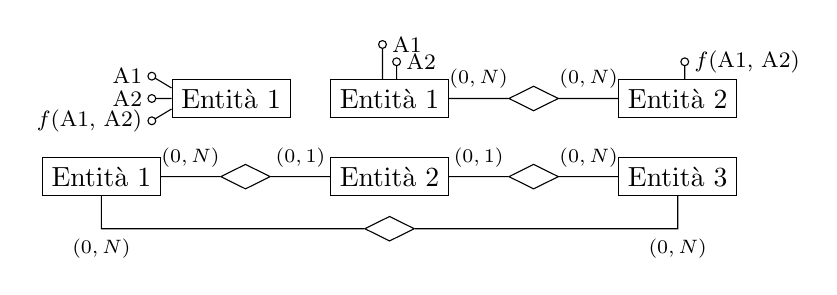
\begin{tikzpicture}
    \draw

    %%* Attributi:
    %%  node[draw, circle, inner sep=1pt,anchor=180, fill=black]{}node[right]{\footnotesize A}
    %%? Distanza orizzontale: E -(0.25,0.x)- A
    %%? Distanza verticale: E -(0,x * 0.22)- A

    %%* Cardinalità:
    %%  node[below right]{\scriptsize $(0,N)$}
    %%  node[above right]{\scriptsize $(0,N)$}
    %%  node[midway, above]{\scriptsize $(0,N)$}

    %%* Relazione:
    %%  node[draw, diamond, shape aspect=2, inner sep=3pt, anchor=90](r1){}
    %%  node[draw, diamond, shape aspect=2, inner sep=0.2pt, anchor=180](r2){R2}

    %%* Entità:
    %%  node[draw, rectangle, anchor=90](e1){}
    %%? Distanza verticale: E -(0.3)- R -(0.3) E
    %%? Distanza orizzontale: E -(0.75)- R -(0.75)- E


    (0,0)node[draw, rectangle, anchor=90](e1){Entità 1}
    (e1.170)--++(-0.25,.15)node[draw, circle, inner sep=1pt, fill=white]{}node[left]{\footnotesize A1}
    (e1.180)--++(-0.25,0)  node[draw, circle, inner sep=1pt, fill=white]{}node[left]{\footnotesize A2}
    (e1.190)--++(-.25,-.15)node[draw, circle, inner sep=1pt, fill=white]{}node[left]{\footnotesize $f($A1, A2)}



    %%* Entità 1
    (e1.0)++(0.5,0)node[draw, rectangle, anchor=180](e1){Entità 1}
    (e1.110)--++(0,0.44)node[draw, circle, inner sep=1pt, fill=white]{}node[right]{\footnotesize A1}
    (e1.70)--++(0,0.22)node[draw, circle, inner sep=1pt, fill=white]{}node[right]{\footnotesize A2}

    %%* Relationship
    (e1.0)--++(0.75,0)node[midway, above]{\scriptsize $(0,N)$}node[draw, diamond, shape aspect=2, inner sep=3pt, anchor=180](r1){}
    % (r1.270)++(0,-0.5)node[align=center]{
    %     $E_1$(\myuline{$A_1$}, $A_2$, $E_1$)\\
    %     $E_2$(\myuline{$A_3$}, $A_4$)
    % }

    %%* Entità 2
    (r1.0)--++(0.75,0)node[midway, above]{\scriptsize $(0,N)$}node[draw, rectangle, anchor=180](e2){Entità 2}
    (e2.70)--++(0,0.22)node[draw, circle, inner sep=1pt, fill=white]{}node[right]{\footnotesize $f($A1, A2)}


    (e1.270)++(0,-0.5)node[draw, rectangle, anchor=90](e2){Entità 2}
    (e2.0)--++(0.75,0)node[midway, above]{\scriptsize $(0,1)$}node[draw, diamond, shape aspect=2, inner sep=3pt, anchor=180](r2){}
    (r2.0)--++(0.75,0)node[midway, above]{\scriptsize $(0,N)$}node[draw, rectangle, anchor=180](e3){Entità 3}
    (e2.180)--++(-0.75,0)node[midway, above]{\scriptsize $(0,1)$}node[draw, diamond, shape aspect=2, inner sep=3pt, anchor=0](r1){}
    (r1.180)--++(-0.75,0)node[midway, above]{\scriptsize $(0,N)$}node[draw, rectangle, anchor=0](e1){Entità 1}
    (e2.270)++(0,-0.25)node[draw, diamond, shape aspect=2, inner sep=3pt, anchor=90](r3){}
    (e1.270)|-(r3.180)node[midway, below]{\scriptsize $(0,N)$}
    (e3.270)|-(r3.0)node[midway, below]{\scriptsize $(0,N)$}
    ;
\end{tikzpicture}
\end{document}